%% APPENDIX B -- the spatial rank as a diagnostic: what it can and cannot
%% support, and the reserved hold-out that calibrates it.
%% Owner: r11-chain.  Carries \label{app:radius} (cited by 04_method.tex)
%% and \label{sec:heldout} (cited from the other appendices).
\section{The spatial rank, and what it can support}
\label{app:radius}

The spatial rank asks whether an excess sits at the star or anywhere else in
the field. It is a diagnostic, no disposition rests on it, and this appendix
is the measurement that settles why: \rankstatus{}

The star lies at the phase centre, inside the control annulus, and the
asymmetry is real. \emph{It is not a primary-beam effect.} Spectra are
extracted from phase-rotated visibilities in apparent flux and are never
corrected for the primary-beam response (Appendix~\ref{app:conventions}), so
the familiar rise of image noise with distance from the pointing centre
cannot operate here; and were it operating, it would make the control probes
noisier than the star and place the stellar rank \emph{above} one half, the
opposite of what is measured. \textbf{No mechanism for the displacement is
established, and we prefer to say so.} What the control ensemble does show is
a weak rise of its own level with radius, and the obvious repair is to remove
it: each probe is standardised within its own radius bin, the radii being
known from the fixed draw, with no free parameter.

\emph{Applied out of sample, the correction does not repair the statistic.}
Frozen --- probe radii, bin edges and standardisation alike --- and applied
unmodified to \RadValStarN{} windows that played no part in its construction,
it moves the median stellar rank from \RadValStarRawMed{} to
\RadValStarCorMed{} against the exchangeable one half, \RadValStarToward{}
it, in both out-of-sample partitions separately. Rescoring the whole survey
with the gradient removed moves the list of crossings outranking all their
controls from \LocStageGlobal{} windows to \LocStageLocal, losing
\LocStageLost{} and gaining \LocStageGained, and leaves the survey median
rank slightly further from one half than before.

The interpretation is narrow and, we think, unavoidable. The radial gradient
is real, but removing it leaves the median no closer to one half, so the
residual is not radial, and neither normalisation yields a calibrated tail
probability. \textbf{We therefore keep the frozen rank --- it has at least
the virtue of having been fixed in advance --- read it only as an indication
of which crossing to examine first, and rest every disposition on physical
evidence or on recurrence.} The radial correction, the region-maximum audit
and the pseudo-star tests each leave every disposition unchanged, and because
the rank gates nothing, none of this enters a sensitivity limit.

\emph{One mechanism can be excluded by measurement, and it is the one that
would matter most.} Equation~\ref{eq:tstar} divides every position by a
single noise scale shared by the star and all its probes. A star bright
enough to carry multiplicative calibration residuals of its own would then
have a noise the shared scale does not describe, and its statistic would be
inflated with nothing in the search to reveal it. The ratio of the two noises
is measurable from the released control vectors alone: because the star and
each probe are divided by the same scale and maximised over the same
channel$\times$drift grid, the stellar statistic divided by the median of
the \NCtrl{} control statistics \emph{is} that ratio, and it is one when the
two noises agree. Over the \NsrNWin{} windows carrying no threshold crossing
its median is \NsrMed{} (star-clustered 95 per cent \NsrLo--\NsrHi), and it
does not climb with the brightness of the field, which is what a
multiplicative error would scale with: \NsrFifthLo{} in the faintest fifth of
control rings against \NsrFifthHi{} in the brightest, and \NsrBrightMed{}
over the \NsrBrightN{} windows whose ring exceeds \NsrBrightSig$\sigma$ and
is therefore set by resolved emission rather than noise. That the ratio
\emph{can} rise is shown by the \NsrCrossN{} windows that do carry a
crossing, where it is \NsrCrossMed. Part of the reason it does not rise
otherwise is structural: a gain error multiplying a continuum raises every
channel of an integration by the same factor, and the per-integration median
along frequency removes exactly that. \textbf{A stellar-position noise
denominator would therefore move no statistic in this survey.}

\subsection{The reserved hold-out, and what it calibrates}
\label{sec:heldout}

The statistic and the mask were settled on the searched sample and cannot
also calibrate themselves, so a hold-out was reserved by a rule fixed and
recorded before any reserved block was searched: a block is held out if and
only if $\mathrm{sha256}(\textsc{uid})_{[:8]} \bmod 5 = 0$, subject to two
guards that use identifiers alone --- a block on the pre-registered list
deposited with this paper stays in the survey, and no system loses every
block --- so that the assignment can be recomputed from the UIDs and that
list alone. The three choices that could manufacture a signal were fixed
before the rule itself: the statistic of Eq.~\ref{eq:tstar}, the trigger and
recurrence criteria, and then the reservation, with the first reserved block
searched \HoLeadBlockDays{} days later. Every diagnostic built afterwards is
incapable of promoting a window.

Of \NEbProcessedAll{} blocks processed, \NEbHeldOut{} are reserved
(\HoPctHeld{} per cent), giving \HoWin{} windows toward \HoStars{} stars with
no star and no system lost from the headline sample. Three quantities are
calibrated on those blocks and on nothing else.

First, the rank displacement. Out of sample the stellar rank has median
\HoRankMed{} where one half is expected, with a block-clustered 95 per cent
interval of \HoRankMedLo--\HoRankMedHi{} over \HoWin{} windows, and
\HOFracLoPct{} per cent of ranks below 0.1 against \HOFracHiPct{} per cent
above 0.9, so the distribution is displaced rather than growing a tail. The
displacement runs the way that matters: a rank below one half places the star
high, and the star in fact outranks all \NCtrl{} probes in \NsrFirstObs{} of
the survey's windows against \NsrFirstExp{} if the positions were
interchangeable. The direction therefore inflates star-first outcomes rather
than suppressing them, which is why the chance expectations of
Appendix~\ref{app:falsealarm} are calibrated on the measured rate.
Clustering removes neither the shift nor its size: \HOBlockBelow{} of
\HOBlockN{} blocks have a mean rank below 0.5, and a star-clustered bootstrap
places the median at \HOBootMed{} (95 per cent \HOBootLo--\HOBootHi). The
searched sample leans the same way without resolving it (median \SurvMedP,
star-clustered 95 per cent \SurvBootLo--\SurvBootHi), and the two
distributions are indistinguishable, so the in-sample checks were
underpowered rather than contradicted. A displacement that survives a
hold-out chosen before the data were seen is a property of the statistic and
not of this sample, and it is the quantitative reason the rank is read as a
diagnostic and never as a significance.

Second, the false-alarm tail factor --- the measured rate at which a
no-signal position ranks first, divided by the rate exchangeability would
give. It is \HoTailFactor{} on \HoPseudoTrials{} trials, with a bootstrap
clustered over the \HoTailBlocks{} reserved blocks giving
\HoTailLo--\HoTailHi. That factor and its width set the accuracy of every
chance expectation in this paper.

The reserved blocks were also searched in their own right, because a
transmitter in them would matter whatever their calibration role: their
\ChnHoWin{} windows hold \ChnHoCross{} threshold crossings, \ChnHoFirst{} of
them outranking all \NCtrl{} controls, and none satisfies the confirmation
criterion.

Third, the radial behaviour of the control ensemble. The standardised
control level runs \HoRadBins{} from the inner to the outer edge of the
annulus, a mean per-window slope of $\HoRadSlope\pm\HoRadSlopeSe$: the
displacement reproduces out of sample, but the steep inner-edge excess seen
in sample does not, so the radial term is small, of the wrong sign to account
for the displacement, and removing it leaves the displacement behind.

The \emph{external calibration sample} must not be confused with the
hold-out, and it is not an out-of-sample set. Its \CampBlocks{} execution
blocks were reserved to calibrate the rank and to supply repeats the hold-out
does not have, and \CalNCensus{} of them are primary-census blocks and
\CalNHoldout{} hold-out blocks, with \CalNOutside{} outside both: it enters no
count of the science sample because its blocks are already counted there, not
because it is external. Over its \CampWindows{} windows the frozen pipeline
returns \CampStageOne{} crossings outranking all their controls ---
\CampStageOneCO{} of them $\beta$~Pictoris CO --- and \CampUnattrib{}
unattributed against \CampExpUn{} expected at the measured tail rate. The
out-of-sample statement this paper makes is the hold-out's, which shares no
execution block with the census.

\subsection{One crossing through the whole chain}
%% (subsection label retired: nothing cites it)

CP$-$72~2713 is the clearest worked example, because every step returns a
verdict rather than a shrug. In Band~7 the crossing reaches
$T_\star=\VnCpT$ in channel \VnCpChan{} of its window; it is unattributed,
with the one nearby transition and its provenance discussed in
Appendix~\ref{app:linemask}; both diagnostics favour it, in that it outranks
every one of the \NCtrl{} control positions and the drift-following
visibility fit puts the emission at the stellar position, ${\rm
Re}/\sigma=\VnCpReAdopted$ against a control-position maximum of
\VnCpCtrlAdopted; and neither of those is a promotion
(\S\ref{sec:vistest}).

\emph{What disposes of it is the repeat block.} The second block matches the
first in tuning, channel width, channel count, integration count and
on-source time, registers to \CpRecOffChan{} of a channel, and is the deeper
of the two, so a persistent emitter at the first block's flux would have
returned $T_\star=\CpRecExpT$ where it returns \CpRecT. Read as two
measurements of one constant amplitude --- the conservative reading, and the
one quoted here --- the pair is inconsistent at $\CpRecExclPair\sigma$. The
blocks are \CpSepH\,h apart, so this is a within-night test: it excludes a
persistent emitter of that strength and says nothing about an intermittent
one. \textbf{The disposition rests on the recurrence test and on nothing
else}, which is the chain applied to every crossing in the survey.

%% ------------------------------------------------------------------
%% NOTE (r11-chain, round 11).  Ruling 2: CP-72 2713 is reported as
%%   UNATTRIBUTED in the primary chain and its disposition is carried by
%%   recurrence, which is what this subsection has always shown.  The SO
%%   coincidence and the provenance of that transition belong to
%%   app_I_linemask.tex (r11-mask) and are referenced, not restated.
%% NOTE (pre-existing, kept for the record): this paragraph once gave
%%   T_star = 5.81 against "a ring maximum of 5.68" and concluded the
%%   crossing "fails the rank screen".  5.81 < 5.68 is false and so was the
%%   conclusion; the statement is now made in the form the rank actually
%%   compares -- the star outranks all \NCtrl controls.
%% DELETED this round to pay for the hold-out paragraph above: the
%%   screen-cost paragraph (12 lines, now moot because the rank gates
%%   nothing), the conditional-reading sigma, and three REQUEST blocks that
%%   had been answered.
%% ------------------------------------------------------------------

%% ★ fig:bpiccontrol MOVED HERE from Sec. 5 in the v4.12 length pass: this
%% appendix is where the spatial statistic is characterised, and the figure is
%% the bound on its reach.  0.36 pp off the main text.
\begin{figure}
\centering
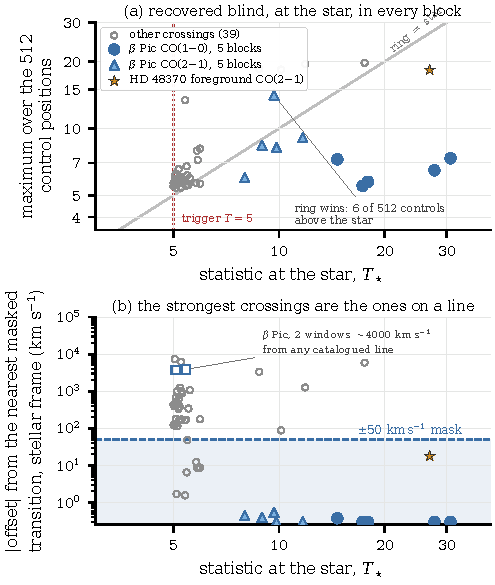
\includegraphics[width=0.88\columnwidth]{figures/bpic_control.pdf}
\caption{The $\beta$~Pictoris positive control, in both directions.
\emph{(a)}~The spatial screen. One point per execution block in which the
blind search recovers circumstellar carbon monoxide, plotted as the stellar
statistic against the maximum over that window's \NCtrl{} control positions:
the \NStageOneBpicEb{} blocks in which the star outranks every control, and
one further block in which the ring wins. \emph{The control is that the
search recovers a real narrow line at a stellar position, in two transitions
and in every one of these blocks.} It is not that the star outranks the ring
everywhere. In block \texttt{\BpCtrlBlock}, Band~\BpCtrlBand, the control
ring reaches \BpCtrlRingMax{} against \BpCtrlStar{} at the star, with
\BpCtrlNAbove{} of the \BpCtrlNCtrl{} control positions above it, so the
screen rejects a window holding carbon monoxide that is real, centred on the
star and independently mapped. The disc is resolved on the scale of the
primary beam in that configuration, which is the geometry the screen is
built to reject, so \textbf{the screen measures compactness and not
authenticity} (\S\ref{sec:bpicval}). \emph{(b)}~Line confusion, which is
what makes the screen's job hard. Each crossing is plotted by its velocity
offset from the nearest masked transition \emph{in its own star's rest
frame}, with the adopted $\pm\MaskHalfKms$\,km\,s$^{-1}$ half-width
marked. The \BpicPanelNCo{} $\beta$~Pictoris carbon-monoxide crossings land
\BpicDvCoLo--\BpicDvCoHi\,km\,s$^{-1}$ from CO, at the resolution of the
systemic velocity itself, while the two CS($5{\to}4$) crossings of the same
star sit \BpicDvCsLo--\BpicDvCsHi\,km\,s$^{-1}$ from anything catalogued
and are not attributed at any width. \BpicPanelNOther{} further crossings
are drawn in grey, with HD~48370 marked; \BpicPanelNDrawn{} of the
\NCross{} are plotted, the remainder being crossings for which the release
stores no control ring. \emph{A crossing is identified by where it falls in
this plane and not by how strong it is}, which is why the line mask and not
the trigger is the productive test.}
\label{fig:bpiccontrol}
\end{figure}
